\documentclass[11pt, oneside]{article}
\usepackage{graphicx}
\usepackage{url}
\begin{document}

\title{The Second Screen}
\author{Michael Fraser}
\maketitle

\begin{abstract}
Devices dubbed ``second screens" have become popular lately, offering new ways of interaction with various systems. This article explores the history and use of second screen technologies to access whether or not these technologies will become staples of future systems. The history of entertainment and television systems with respect to using second screens are the primary focus, as they suggest the future of the technology. The accessibility, efficiency, and satisfaction associated with second screen systems are explored to produce a hypothesis on the future of the second screen technologies.
\end{abstract}
% JD: I think you mean "to *assess* whether or not..." in the second sentence above.
%     The abstract puts me on guard...remember, this is a *mental model* paper, not
%     a generalized technology review.  We'll see.

\tableofcontents

\section{Introduction}
Almost everyone these days has a tablet or smartphone device. As the various forms of media begin to recognize this fact, they begin to utilize it to their advantage. It used to be that people would sit down and watch TV with whatever TV screen they had at the time, and interaction with their favorite TV show was limited to this action. As technology advanced, the common TV watcher was granted easy accessibility to a second screen of sorts: a tablet or smartphone. 

The same is true for users of entertainment systems and computers; multiple screens are available to push the limits of interaction with common devices. Applications and devices are now able to allow for a more in-depth interaction with the systems people have interacted with in a limited way for so long. Are these so called ``second screens" going to replace the traditional forms of interaction with common systems, or will it remain a specialized tool for specific applications?

\section{Background}

\subsection{Computers}
Computers have had the capability to connect to multiple screens since the late 90's. As computers have advanced technologically though, applications for a second monitor have stayed relatively the same: a larger space to spread around programs and applications. An example illustrating a multi-monitor computer system can be seen in Figure \ref{monitors}. Multiple monitors do not follow with the second screen ideology discussed here, as multiple monitors are mostly used as a single, larger screen rather than two separate systems. Computers can still be part of second screen systems though, as the computer could interact with a phone, tablet, or even a TV. For this article, computers as part of second screen systems will not be discussed much further.

\begin{figure}
    \centering
    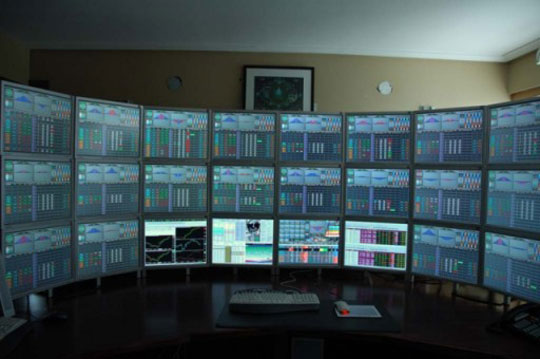
\includegraphics[width=.8\textwidth]{Multiple-Monitor-Setup.jpg}
    \caption{A 24-monitor computer system.}
    \label{monitors}
\end{figure}

\subsection{Entertainment Systems}
% JD: Ideally, even historical notes should have cited sources, especially for
%     information that is not common knowledge.
A second screen application can also be found with the top entertainment systems as well. Systems as early as the Dreamcast were making use of a second screen to add more interaction between the user and the games they play. With the Visual Memory Unit (VMU), Dreamcast users could download mini-games that could be played separately and later incorporated back into the game. The GameCube was the next to utilize a second screen by allowing users to connect a Game Boy Advance to the console. By connecting two games, the user could share file information or items and have it directly affect both games simultaneously. 

The Wii U was released to work alongside the Wii, allowing users a second screen to utilize while playing their favorite game. The Wii U controller had the second screen that allowed users to perform secondary tasks, such as select something from inventory or view a map. Soon after, Microsoft unveiled the Xbox SmartGlass, designed to work with the Xbox 360 to allow easier interaction with the console. Instead of producing a new device for the second screen, Microsoft utilized the technology that users already have: their smartphones and tablets. The Xbox SmartGlass is an app for the Iphones, Android phones and tablets, and Windows 8 devices \cite{MashableSmartGlass}.

Table \ref{entertainment_table} shows a list of primary and secondary screens that entertainment systems have used to increase interactivity with video games. 

%Playstation shortened to PS because otherwise the table size became a latex warning and would not center itself correctly.
\begin{table}
    \centering
    \caption{List of primary and secondary screens for entertainment systems \cite{wiki_second_screen}.}
    \begin{tabular}{| c | c |}
        \hline
        Primary Screen & Secondary Screen \\ \hline
        Dreamcast & VMU \\ \hline
        GameCube & Game Boy Advance \\ \hline
        PlayStation 3 & PS Portable and Vita using Remote Play \\ \hline
        Playstation 4 & PS Vita Remote Play; iOS, Android with PS App \\ \hline
        Wii & Nintendo DS \\ \hline
        Wii U & Wii U GamePad and Nintendo 3DS \\ \hline
        Xbox 360 & Smartphones and Tablets with Xbox SmartGlass\\ \hline
        Xbox One & Smartphones and Tablets with Xbox SmartGlass \\ \hline
    \end{tabular}
    \label{entertainment_table}
\end{table}

\subsection{Television} 
Second screen development is most common with televisions, where tablets or smartphones are used to connect users to their shows in an alternative way. The users view the programs and use their second screens to answer questions or find out more details about a particular scene. Figure \ref{second-screen} shows a tablet displaying the same program as the TV, an example of an application of second screen technologies. Since the development of social networking sites like Facebook and Twiter, the media has been engaging their supporters through mass messages. Prime time shows like Covert Affairs post statuses on the show's facebook page engaging followers about the decisions made in the show, whereas shows like Tosh.0 have the host direct the viewers into tweeting about things Tosh has said or done. 
% JD: OK, so far, this is a technology survey.  Necessary for this topic, but it should
%     have a supporting role.

\begin{figure}
    \centering
    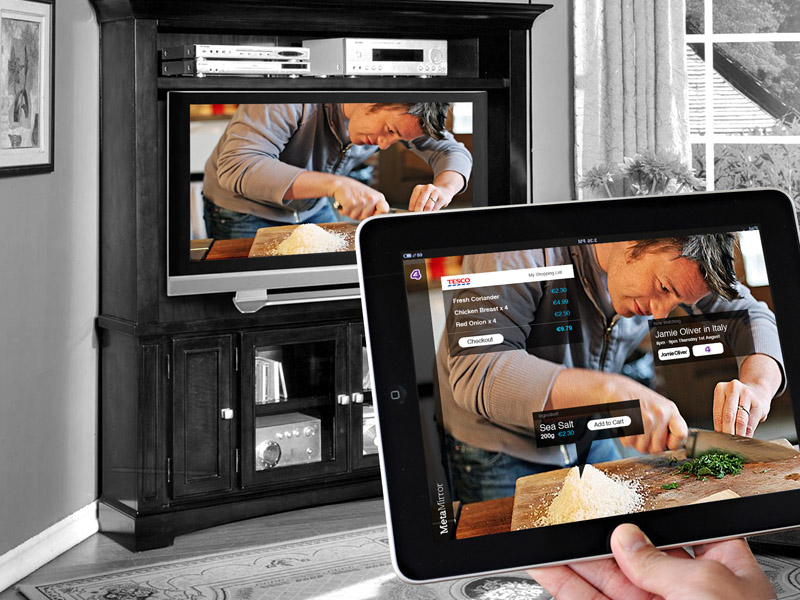
\includegraphics[width=.8\textwidth]{second-screen.jpg}
    \caption{Example of the second screen with respect to TV [Image from advanced-television.com].}
    \label{second-screen}
\end{figure}

Studies completed by Twitter have found that when a show is airing that directly integrates tweets into the content, there is a major increase in the number of tweets engaging the show's hashtag subjects \cite{TwitterTV}. Chris Gorham of Covert Affairs was interviewed by Mashable on the effects of the second screen and the show's success. He believes Twitter is a way of sharing the behind-the-scenes process with his fans \cite{MashableChris}. Not all discussions about television shows on social networking sites start with the show's page though. While social networking provides the means for interaction with shows, it turns out that audiences are actually creating forums for inter-audience discussion on their own \cite{ACM}.
% JD: Plus, Twitter strikes me as an "incidental" second screen---it just happens
%     to be available.  There is nothing about its interaction design that (to me)
%     tailors it for use as a second screen.

Second screen technologies provide potential social benefits as well with new applications of the devices. The usefulness of a second screen was tested with a subtitle and sign-language system, where subtitles or sign language corresponding to a TV show were produced on the second screen \cite{IEEE_EFS}. While the program provided the sign language and subtitles for the viewed program, it was found that syncing the TV screen and second screen TV was difficult. An illustration of how the second screen provided sign language for a program can be found in Figure \ref{sign-language}.
% JD: Haha, OK, now you answered my question :)

\begin{figure}
    \centering
    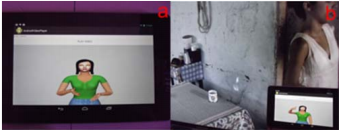
\includegraphics[width=.8\textwidth]{SignLanguage.png}
    \caption{Example of how a second screen can be used to improve the viewability of TV \cite{IEEE_EFS}.}
    \label{sign-language}
\end{figure}

\section{Methods}
A simple Google search reveals that this is not a new concept. Hundreds of articles or blog posts can be found on the topic of second screen, all revolving around the TV, the media, or entertainment systems. To investigate whether or not the second screen was here to stay, searches were done in the IEEE Xplore and ACM digital libraries along with simple web searches. Simple web searches yielded blog entries from Twitter and Mashable, along with a page of history on the second screen technologies from Wikipedia.

The blogs cited above are both well known and significant in the media. Twitter's blog would be very authoritative when it comes to social networking discussions, as Twitter itself is a social networking site. Mashable is not a social networking site, but is a technology blog which discusses current technological advances in the media. The articles from Mashable discuss the use of social networking to allow for increased interaction between users and TV program content. 

The digital libraries cited above are two of the top digital libraries dealing with technology. The article from ACM supports the blogs discussions on social networking and it's importance in the development of the second screen. The article from IEEE provides an alternative use for second screen technologies: using them to support disabled persons and allow them to view TV programs they may be otherwise incapable of doing.

The sources have a mix of technical and social backgrounds, yet they all support the others. In this way, there is a common authority split among them. The views agree that social networking is a big part of second screen development, and seem to suggest that more development with second screen technologies is underway.
% JD: Ohhhkay, this is all well and good so far, but take note of the focus.
%     We want to explore second screens from an interaction design perspective,
%     particularly on the mental model of users who wish to consume their entertainment
%     with a second screen.  In fact it would be valid to ask whether most users even
%     *want* such an experience.  We'll see with what remains of the paper...

\section{Discussion}

\subsection{Entertainment Systems}
The fact that entertainment systems trace back to the Dreamcast for second screen technologies suggests that the technology will not be fading away anytime soon. Also of significance is the recent increase in second screen technologies, as the three major current entertainment systems support second screens. From analyzing this data alone, it is clear that second screen technologies will only continue to develop further.
% JD: This assertion is not very well-founded.  It could be a fad (with the exception
%     of the Dreamcast).  You need something more solid to back this claim.

Second screens in the field of entertainment systems add a certain level of satisfaction that stems from the video gaming culture. Having a single technological device that can provide the services of many different devices is convenient and efficient. There is no need to worry about becoming proficient with a new device either, as the devices people use commonly in their lives like their smartphones or tablets are already well understood by the user. A new function for a decently expensive device just makes the cost of the device that much more worthwhile as well, which again leads to a higher satisfaction rating for the device. 

Second screen technologies with entertainment systems are even more successful when they replace previously inefficient or confusing interfaces, such as the way the YouTube application on the Xbox 360 has a difficult keyboard to use with a controller. Instead, a user may use their phone to type the search criteria of the video they are looking for and get the process done quickly. This example illustrates the efficiency of the XboxGlass feature to use the keyboard for writing text that the console will use. 
% JD: OK, this paragraph is finally getting to where I hoped most of the paper would be.

The success of the second screens when used with entertainment systems stems from satisfaction and efficiency/ease of use. If people are happy with a product, they will continue to utilize and support that product. If a second screen application increases the satisfaction with an entertainment system, then users will be more willing to include second screen applications in their use of the system. The satisfaction levels directly relate to the utility of the application or device, as if the application assists with a otherwise bothersome task, then the user will be happier overall when engaging that task. When done properly, a second screen device could change the way users interact with entertainment systems drastically.
% JD: The discussion here is almost circular.  People will use something if they like it;
%     people like it if it's useful.  You should start with a need.  What need does a
%     second screen address?  Is it a valid need?  Is the need addressed well?  This
%     should be the track that you're on.

\subsection{Television}
\subsubsection{The User's Perspective}
For television systems and TV program content, social networking is key. Social networking applications on tablets or smartphones allow for easy access to content corresponding to TV programs. Users will discuss events of a show between themselves or communicate with people of the show directly, allowing the show to display those thoughts live. There is a certain level of excitement and satisfaction that users certainly gain from seeing their 'tweet' appear on TV, just as there is a small human desire to be well-known or famous. Big fans of TV programs may also just enjoy the more in-depth discussion of the show, as other fans may bring conflicting opinions of a show event to light.
% JD: Any sources for this?  In any case, you have a lead here.  The idea of a shared
%     viewing experience is very compelling.  Live theater, live music, and traditional
%     cinema (sort of) have these characteristics.  This is good; this can ground you.
%     But now you have to apply this to the "system image" that the second screen provides.

With the age of smartphones, TV audiences hardly have to move to indulge in second screen show content. All they need is their phone, which people tend to have on them at all times. There are high levels of satisfaction with using a phone as a remote as well, as there is satisfaction with using any one tool to do multiple jobs. Misplaced phones are typically easily located as well, whereas remote controls have no easy way of being found.
% JD: Phones as smart remotes is another good lead.  But you're stopping short.  This
%     is where you should dive in.  This is where you need lots of references.

An advantage social networking would have over new softwares is the familiarity of use that users already have with social networking applications. There is no new process of learning that a user must undergo, as they will be able to remember how they have interacted with the application previously. Social networking sites are already developed with interaction design principles, and have been improving over time. A new software or application would need to work up to those levels of design before having the chance of being successful.
% JD: As mentioned earlier, this can be good and bad.  Nice that they are familiar;
%     however, as second screens, they come across as incidental.  Is that OK?  Or can
%     that be improved?

\subsubsection{The Media's Perspective}
The media is realizing the potential of second screen devices and embracing it. Commercials are already informing viewers about Twitter hashtags, like T.J.Maxx's ``\#Maxxinista," where users can find more products that T.J.Maxx has for sale. As stated before, television shows like Covert Affairs use the second screen applications like Twitter to better connect with their users, and Tosh of Tosh.0 directly incorporates tweets from users into his show. Any sign of viewer interest is good news for show producers, and Twitter provides a new channel for viewers to express interest. 

Encouraging social networking messages would also increase the average number of viewers per episode, as the social networking would remind the fans to watch the show each night. On another level, social networking sites often allow users to view items corresponding to their friends activities. This provides an opportunity to find new fans as users of networking sites become interested in their friends activities.

As audiences create their own forums to discuss TV shows, the media will take note on what to bring to discussion themselves and how to better engage their audience. New ways to discuss the shows will be developed also, as the media begins to better incorporate themselves into the messaging process. Alternatively, social networking sites like Twitter will modify themselves to better accommodate the second screen traffic corresponding to TV shows. 
% JD: OK, see, you're painting a picture here.  It has potential.  This can be the
%     basis for a "second screen mental model."  What do users expect?  What level
%     of interaction with others is ideal?  What metrics are important?
%
%     But unfortunately, we are now at the conclusion...

\section{Conclusions}
Second screen technologies have been around for a while, but still have plenty of room to grow. Applications already exist for television and entertainment systems that incorporate second screen technologies. These applications allow more direct interaction with the content of the different systems, providing more control to the user, which in turn increases the satisfaction associated with that system and the second screen device. 
 
With entertainment systems, increased satisfaction and efficiency that second screen devices offer suggest that second screen applications will continue to be developed with current and future generations of video game consoles. With second screen support already announced with the next generation consoles, it seems the technology will continue to be developed. 
% JD: This paragraph strikes me as needing better support.  It's just saying that
%     the second screen will stay because they are being made.  A little weak.

For television systems and shows, second screen technology and social networking are already at work connecting users to show content. As users tend to be creating forums for the discussion of shows on their own, it is obvious that this technology will continue to grow. Secondary applications of second screen devices are also under development, such as an application to produce sign language imagery or subtitles corresponding to what is said in a show. These secondary applications are important in that they allow all users to share in the experience of a TV show which would normally exclude many individuals.

With new applications being developed and high satisfaction levels for the applications that are already developed, it is very likely that second screen technologies are here to stay. Second screen technologies are not too limited in potential either, as can be gleaned by the shear number of uses a smartphone or tablet has. As attention turns toward second screen devices, everyone can expect to see newer and greater applications of this technology in the near future.
% JD: Some presumptiveness here too.  Ultimately, I think where you left off in
%     the previous section is just the beginning.  You can potentially shorten
%     the history and product review, then do more reading on usability issues
%     pertaining to the second screen.  That's really where we want this paper
%     to play.  Your initial set of references is a good start, but I can imagine
%     that there are more out there, now focusing on usability issues.  *That* is
%     the intended focus of this "mental model" paper.

\bibliography{mental.bib}{}
\bibliographystyle{plain}

\end{document}
